% This is samplepaper.tex, a sample chapter demonstrating the
% LLNCS macro package for Springer Computer Science proceedings;
% Version 2.21 of 2022/01/12
%
\documentclass[runningheads]{llncs}
%
\usepackage[T1]{fontenc}
% T1 fonts will be used to generate the final print and online PDFs,
% so please use T1 fonts in your manuscript whenever possible.
% Other font encondings may result in incorrect characters.
%
\usepackage{graphicx}
% Used for displaying a sample figure. If possible, figure files should
% be included in EPS format.
%

\usepackage{hyperref}
%\usepackage{multicol}
%\usepackage{footmisc}
%\usepackage{amstext}
\usepackage{amsmath}
\usepackage{amssymb,stmaryrd}
\usepackage{mathrsfs}
\usepackage{mathtools}
%\usepackage{amsthm}
\usepackage[english]{babel}
%\usepackage[official,right]{eurosym}
\selectlanguage{english}
\hyphenation{ExecEngine DevOps}
%\newtheorem{lemma}{Lemma}


% Ampersand -----------------------------------------------------------

%\def\id#1{\text{\it #1\/}}
\newcommand{\xrightarrowdbl}[2][]{%
  \xrightarrow[#1]{#2}\mathrel{\mkern-14mu}\rightarrow
}
\newcommand{\id}[1]{\text{\it #1\/}}
\newcommand{\code}[1]{\text{\tt\small #1}}
\newcommand{\stmtText}[1]{``{\small\tt #1}''}
\newcommand{\dom}[1]{\id{dom}(#1)}
\newcommand{\cod}[1]{\id{cod}(#1)}
%\renewcommand{\int}[2]{\id{inter}(#1,#2)}
\newcommand{\relsIn}[1]{\id{relsIn}(#1)}    % maps a Term to a set of Relations
\newcommand{\popF}[1]{\id{pop}_{#1}}
\newcommand{\pop}[2]{\popF{#1}(#2)}
\newcommand{\maintain}{\mathbin{\id{maint}}}
\newcommand{\enf}{\mathbin{{\tt enforce}}}
\newcommand{\enforce}[2]{{\tt enforce}_{#1}(#2)}
\newcommand{\instance}{\mathbin{\id{inst}}}
\newcommand{\relname}[1]{\id{relname}(#1)}
\newcommand{\evt}[2]{\id{event}_{#1,#2}}
\newcommand{\src}[1]{\id{src}(#1)}
\newcommand{\tgt}[1]{\id{tgt}(#1)}
\newcommand{\viol}[2]{\violC{#1}(#2)}
\newcommand{\violC}[1]{\id{viol}_{#1}}
\newcommand{\sign}[1]{\id{sign}_{#1}}
\newcommand{\enfRel}[1]{\id{enf}_{#1}}
\newcommand{\signature}[2]{\langle{#1},{#2}\rangle}
\newcommand{\powerset}[1]{\cal{P}\{#1\}}
\newcommand{\la}{\langle}
\newcommand{\ra}{\rangle}
\newcommand{\full}{V}
\newcommand{\declare}[3]{\id{#1}_{\pair{#2}{#3}}}
\newcommand{\subst}[3]{#3_{[#1\rightarrow #2]}}
\newcommand{\fullt}[2]{V_{\pair{#1}{#2}}}
\newcommand{\iden}{I}
\newcommand{\ident}[1]{I_{\id{#1}}}
\newcommand{\expr}[3]{(#1)_{#2\times #3}}
\newcommand{\pair}[2]{\langle{#1},{#2}\rangle}
\newcommand{\maprel}[2]{{\tt maprel}_{#1}({#2})}
\newcommand{\Pair}[2]{#1\times#2}
\newcommand{\pairs}[1]{\id{pairs}(#1)}
\newcommand{\triple}[3]{\langle{#1},{#2},{#3}\rangle}
\newcommand{\quintuple}[5]{\langle{#1},{#2},{#3},{#4},{#5}\rangle}
\newcommand{\atom}[1]{{\tt\small #1}}
\newcommand{\atoms}{\mathcal{A}}
\newcommand{\Atoms}{\mathbb{A}}
%\newcommand{\events}{\mathcal{E}}
%\newcommand{\Events}{\mathbb{E}}
\newcommand{\concept}[1]{{\tt\small #1}}
\newcommand{\concepts}{\mathcal{C}}
\newcommand{\Concepts}{\mathbb{C}}
\newcommand{\decls}{\mathcal{D}}  %% names of relations
\newcommand{\rels}{\mathcal{R}}   %% all relations
\newcommand{\Rels}{\mathbb{R}}   %% all relations
\newcommand{\relations}{\mathcal{M}} % representing terms. M is a subset of R.
\newcommand{\triples}{\mathcal{T}}
\newcommand{\Triples}{\mathbb{T}}
\newcommand{\Triple}[3]{#1\times#2\times#3}
\newcommand{\vertices}{N}
\newcommand{\rules}{\mathcal{U}}
\newcommand{\transactions}{\mathcal{E}}
\newcommand{\busConstraints}{\mathcal{B}}
\newcommand{\Constraints}{\mathbb{U}}
\newcommand{\specrules}{\mathcal{S}}
\newcommand{\roles}{\mathcal{O}}
\newcommand{\dataset}{\mathscr{D}}
\newcommand{\Dataset}{\mathbb{D}}
\newcommand{\schema}{\mathscr{Z}}
\newcommand{\functionality}{\mathscr{F}}
\newcommand{\select}[2]{\id{select}_{#1}\{{#2}\}}
\newcommand{\migrsys}{\mathscr{M}}
\newcommand{\infsys}{\mathscr{S}}
\newcommand{\tf}[1]{\mathscr{T}(#1)}
\newcommand{\ptf}[1]{\mathscr{T}'(#1)}
\newcommand{\ti}[1]{\mathscr{I}(#1)}
\newcommand{\tic}[1]{I_{\cal C}(#1)}
\newcommand{\relAdd}{\dagger}
\newcommand{\flip}[1]{{#1}^\smallsmile} %formerly:  {#1}^\backsim
\newcommand{\kleeneplus}[1]{{#1}^+}
\newcommand{\kleenestar}[1]{{#1}^*}
\newcommand{\cmpl}[1]{\overline{#1}}
\newcommand{\rel}{\times}
\newcommand{\compose}{;}
\newcommand{\subs}{\subseteq}%{\models}
\newcommand{\fun}{\rightarrow}
\newcommand{\isa}{\preceq}
%\newcommand{\isaClos}{\sqsubseteq}
\newcommand{\typetest}{?}
\newcommand{\meet}{\sqcap}
\newcommand{\join}{\sqcup}
\newcommand{\Meet}{\bigsqcap}
\newcommand{\Moin}{\bigsqcup} % because LaTeX has already defined command \Join.
\newcommand{\order}{\ominus}
\newcommand{\anything}{\top}
\newcommand{\nothing}{\bot}
\newcommand{\rewriteto}{\rightarrow}
\newcommand{\calc}{\implies}
\newcommand{\alland}{\bigwedge}
\newcommand{\mph}[3]{#1_{#2\times #3}}
\newcommand{\mphu}[1]{#1_{\univ\times\univ}}

%-----------------------------------------
\newcommand{\kse}{\hspace*{1.7em}}
\newcommand{\ksf}{\hspace*{1em}}
\newcommand{\ksg}{\hspace*{1em}}
\newenvironment{derivation}{\begin{tabbing}\kse \= \ksf \= \ksg \= \kill}{\end{tabbing}}
%\newtheorem{definition}{Definition}
\newcommand{\term}[1]{\>\>\(#1\)\\[1ex]}
\newcommand{\rela}[2]{\>\(#1\)\>\>\{ \ #2 \ \}\\[1ex]}
\newcommand{\weg}[1]{}

\def\define#1{\label{dfn:#1}{\em #1}\index{#1}}
\def\definem#1{\label{dfnm:#1}{\em #1}\index{#1}\marge{#1}}
\newcommand{\marg}[1]{\index{#1}\marge{#1}}



\usepackage{color}
\renewcommand\UrlFont{\color{blue}\rmfamily}
%
\begin{document}
%

\title{Data Migration under a Changing Schema in Ampersand}
%
%\titlerunning{Abbreviated paper title}
% If the paper title is too long for the running head, you can set
% an abbreviated paper title here
%
\author{Sebastiaan Joosten\inst{1}\orcidID{0000-0002-6590-6220}\\ \and
Stef Joosten\inst{2,3}\orcidID{0000-0001-8308-0189}}
%
\authorrunning{S. Joosten}
% First names are abbreviated in the running head.
% If there are more than two authors, 'et al.' is used.
%
\institute{University of Minnesota, Minneapolis, USA \and Open Universiteit, Heerlen, the Netherlands\\ 
\email{stef.joosten@ou.nl} \and
Ordina NV, Nieuwegein, the Netherlands}
%
\maketitle              % typeset the header of the contribution
%
\begin{abstract}
   Software generators that compile and deploy a specification into a functional information system
   can help to increase the frequency of releases in the software process.
   They achieve this by reducing development time and minimizing human-induced errors.
   However, many software generators lack support for data migration.
   This can inhibit a steady pace of releases, especially for increments that alter the system's schema in production.
   Consequently, schema-changing data migrations often face challenges, leading developers to resort to manual migration or employ workarounds.

   To address this issue, this paper proposes a foundational theory for data migration,
   aiming to generate migration scripts for automating the migration process.
   The overarching challenge is preserving the business semantics of data amidst schema changes.
   Specifically, this paper tackles the task of generating a migration script based on the schemas of both the existing and the desired system,
   under the condition of zero downtime.
   The proposed solution was validated by a prototype demonstrating its efficacy.
   Notably, the theory is technology-independent, articulating systems in terms of invariants, thereby ensuring applicability across various scenarios.
   The migration script generator will be implemented in a software generator named Ampersand.
\keywords{Generative software \and Incremental software deployment \and Data migration \and Relation algebra \and Ampersand \and Schema change \and Invariants \and Zero downtime}
\end{abstract}

\section{Introduction}
\label{sct:Introduction}
   In practice, information systems%
   \footnote{In the sequel, the word ``system'' refers to the phrase ``information system'', to simplify the language a little.}
   may live for many years.
   After they are built, they need to be updated regularly to keep up with changing requirements in a dynamically evolving environment.
   Schema changes cannot always be avoided when updating software, so a \define{schema-changing data migration} (SCDM) will be neccessary from time to time.
   For example, adding or removing a column to a table in a relational database adds to the complexity of migrating data.
   Even worse, if a system invariant changes, some of the existing data in the system may violate the new invariant.
   In practice, data migrations typically follow Extract-Transform-Load (ETL) patterns~\cite{Theodorou2017},
   for which many tools are available.
   However, ETL tools typically provide little support for invariants that change, forcing development teams to write code.
   In a world where automation of the software process is resulting in higher productivity, more frequent releases, and better quality,
   SCDM's should not stay behind.
   Roughly half of the DevOps~\cite{BassWeberZhu15} teams that responded in a worldwide survey in 2023~\cite{HumanitecDevOps2023} are deploying software more frequently than once per day.
   Obviously, these deployments are mostly updates of existing systems.
   The risk and effort of SCDMs explains why these teams try to avoid schema changes in the first place.
   Our research aims at automating SCDMs to make them less risky and less costly,
   so development teams can deploy schema changes with zero downtime.

   Data migration for other purposes than schema change has been described in the literature.
   For instance, if a data migration is done for switching to another platform or to different technology,
   e.g.~\cite{Gholami2016,Bisbal1999},
   migration engineers can and will avoid schema changes and functionality changes
   to avoid introducing new errors in an otherwise error-prone migration process.
   In another example, Ataei, Khan, and Walkingshaw~\cite{Ataei2021,Walkingshaw2014} define a migration as a variation between two data structures.
   They show how to unify databases with slight variations by preserving all variations in one comprehensive database.
   This does not cater for schema changes, however.
   Then there are SCDMs in situations without a schema or an implicit schema, e.g.~\cite{Hillenbrand2022}.
   Such situations lack the error preventing power that explicit schemas bring during the development of software.
   All errors a schema can prevent at compile time must then be compensated by runtime checks,
   which increases the likelyhood of end-users getting error messages.
   This requires versioned storage of production data and an overhead in performance.
   That is why this paper focuses on SCDMs for systems with an explicit schema.
   The prototypical use case for that is to release updates of information systems in production,
   where the semantic integrity of data must be preserved across schema changes.
   Another use case is application integration for multiple dispersed data sources with explicit schemas.

   A practical complication in many data migration projects is the presence of deteriorated data.
   To clean it up may incur much work.
   Some of that work must be done before the migration; some can wait till after the migration.
   In all cases, data pollution in an existing system requires careful analysis and planning.
   We can capture the automatable part of the data quality problem by regarding it as a requirement to satisfy semantic constraints.
   E.g. the constraint that the combination of street name, house number, postal code, and city occurs in
   a registration of valid addresses can be checked automatically.
   In a formalism like Ampersand~\cite{JoostenRAMiCS2017,Joosten-JLAMP2018}, which allows us to express such constraints, we can add constraints for data quality to the schema.
   This allows us to signal the data pollution at runtime.
   Some forms of data pollution are not automatable, however.
   An example is when a person has deliberately specified a false name without violating any constraint in the system.

   The complexity of data migration has prompted us to develop a theory first,
   which we present in this contribution.
   We have validated the theory by prototyping because a formal proof of correctness is currently beyond our reach.
   This theory perceives an information system as a data set with constraints,
   so we can represent invariants (and thus the business semantics) directly as constraints.

   The next section analyzes SCDMs with an eye on zero downtime and data quality.
   It sketches the outline of a procedure for SCDMs.
   Section~\ref{sct:Definitions} formalizes the concepts that we need to define the procedure.
   Section~\ref{sct:Generating} defines the algoritm for generating a migration system, to automate SCDMs.
   Section~\ref{sct:PoC} demonstrates the prototype of a migration system, which we used to validate our theory experimentally.
   For this purpose we have used the language Ampersand
   because its syntax and semantics correspond directly to the definitions in section~\ref{sct:Definitions}.

\section{Analysis}
\label{sct:Analysis}
   This section analyzes information systems qualitatively, to prepare for a formal treatment in section~\ref{sct:Definitions}.
   The current section yields a procedure for migrating data from one system to another.
\subsection{Information Systems}
   The purpose of an information system is to store and disclose data in a way that is meaningful to its users.
   Multiple users, working from different locations and on different moments, constitute what we will loosely call ``the business''.
   The data in the system constitutes the collective memory of the business,
   which relies on the semantics of the data to draw the right conclusions and carry out their tasks.
   \begin{figure}[bht]
      \begin{center}
        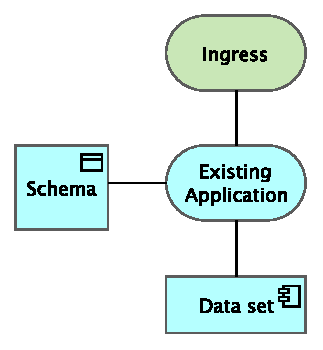
\includegraphics[scale=0.8]{figures/existing system.pdf}
      \end{center}
   \caption{Anatomy of an information system}
   \label{fig:pre-migration}
   \end{figure}
   
   Figure~\ref{fig:pre-migration} depicts the situation before migration.
   An existing application service ingests traffic through an ingress and persists data in a data set, which is typically a database.
   Our research assumes that the structure and business semantics are represented in a schema, from which the system is generated.
   Actors (both users and computers) are changing the data in a system continually.
   The state of the system is represented by a data set, typically represented in some form of persistent store such as a database.
   Events that the system detects may cause the state to change.
   To keep our theory technology independent, we assume that data sets contain triples.
   This makes our theory valid for every kind of database that triples can represent,
   including SQL databases, object-oriented databases, graph databases, triple stores, and other no-SQL databases.

   We assume that constraints implement the business semantics of the data.
   Constraints represent business concerns formally, so they can be checked automatically and can be used to generate software.
   Some of the constraints require human intervention, while others require a system to intervene.
   In this paper, we distinguish three different kinds of constraints:
\begin{enumerate}
\item Blocking invariant\\
   A \define{blocking invariant} is a constraint that is always true in a system.
   It serves to constrain the data set at runtime.
   When the data set changes in a way that violates a blocking invariant, the system produces an error message and refuses the change.
\item Transactional invariant\\
   The classical database transaction can be understood as a \define{transactional invariant},
   which the system keeps satisfied by adding or deleting triples to the dataset.
   As soon as the data violates this constraint, the system restores it without human intervention.
   So, the outside world experiences this as a constraint that is always true, i.e.~an invariant.
\item Business constraint\\
   A \define{business constraint} is a constraint that users can violate temporarily until someone restores it.
   Example: ``An authorized manager has to sign every purchase order.''
   Every violation requires some form of human action to satisfy the business constraint (e.g. "sign the purchase order").
   That takes some time, during which the constraint is violated.
   So, we do not consider business constraints to be invariants.
\end{enumerate}
   Summarizing, in our notion of information systems, concepts, relations, and constraints carry the business semantics.
   Of the three types of constraint, only two are invariants. 

\subsection{Ampersand}
   We employ Ampersand as a prototyping language to demonstrate our theory.
   More significantly, our intention is to augment the Ampersand compiler with the theory outlined in this paper
   to generate migration systems automatically.

   Ampersand serves as a language for specifying information systems through a framework of concepts, relations, and constraints.
   It encompasses the necessary constraints discussed in this paper, making it an ideal platform for practical testing of our theory.
   In Ampersand, developers articulate constraints using heterogeneous relation algebra~\cite{Hattensperger1999,Alloy2006}
   The systems they generate maintain invariants and alert users to violations of business constraints.
   Ampersand's explicit representation of all invariants in its source code makes it well-suited for implementing our theory.
   The absence of imperative code in Ampersand scripts enhances system reasoning,
   while its static typing~\cite{vdWoude2011} yields the established benefits in software engineering processes~\cite{HanenbergKRTS14,Petersen2014}.
   Constraints, which carry business semantics, make ``preserving the meaning as much as possible'' explicit.
   An Ampersand script provides just enough information to generate a complete system,
   allowing extraction of a classical database schema (i.e., data structure plus constraints) from the Ampersand script.

   Ampersand has seen practical use both in education (Open University of the Netherlands) and industry (Ordina and TNO-ICT).
   For instance, Ordina developed a proof-of-concept of the INDIGO-system in 2007,
   leveraging Ampersand for accurate results under tight deadlines.
   Today, INDIGO serves as the core information system for the Dutch immigration authority (IND).
   More recently, Ampersand played a role in designing the DTV information system for the Dutch Food Authority (NVWA),
   with a prototype built in Ampersand serving as a model for the actual system.
   TNO-ICT, a prominent Dutch industrial research laboratory, has utilized Ampersand for various research purposes,
   including a study of international standardization efforts of RBAC (Role-Based Access Control) in 2003,
   and a study of IT architecture (IEEE 1471-2000)\cite{IEEE1471} in 2004.
   Ampersand has also been employed at the Open University of the Netherlands,
   where it is taught in a course called Rule-Based Design\cite{RBD}.
   Students in this course utilize a platform named RAP, constructed in Ampersand~\cite{Michels2015},
   which represents the first Ampersand application to run in production.

   \subsection{Zero downtime}
   To make the case for zero downtime, consider this problem:
   Suppose we have an invariant, $u$, in the \define{desired system}, which is not part of the \define{existing system}.
   In the sequel, let us call this a \define{new invariant}.
   Now, suppose the data in the existing system does not satisfy $u$.
   If $u$ is a transactional invariant, the desired system will restore it automatically.
   But if it is a blocking invariant, the desired system cannot spin up because all of its invariants must be satisfied.
   To avoid downtime, we must implement new blocking invariants initially as a business constraint,
   to let users satisfy them.
   The moment the last violation of $u$ is fixed, the business constraint can be removed and $u$ can be implemented as a blocking invariant.
   This is the core idea of our theory.

   The \define{migration system} to be generated is an intermediate system,
   which contains all concepts, relations, and constraints of both the existing and the desired system.
   However, it implements the blocking invariants of the desired system as business constraints.
   This migration system must also ensure that every violation that is fixed is blocked from recurring.
   In this way, the business constraint gradually turns into a blocking invariant, satisfying the specification of the desired system.
   Since the number of violations is finite, the business can resolve these violations in finite time.
   In this way, the migration system bridges the gap and users get a zero downtime SCDM.

   Summarizing, the following requirements apply to SCDMs
\begin{enumerate}
\item users must experience zero downtime, to enable more frequent SCDMs.
\item users must be able to fix invariants in the new system.
   So, we need an intermediate ``migration system'' that implements blocking constraints of the desired system as business constraints,
   in order to deliver zero downtime.
\item the number of violations that users must fix is finite and decreases (monotonically) over time,
   to ensure that the migration system does not need to live ever after.
\end{enumerate}

\subsection{Data Migrations}
   Data migration occurs when a desired system replaces an existing one,
   while preserving the meaning of the present data as much as possible~\cite{Spivak2012}.
   %Just copying the set of data from the existing system to the desired system is obviously wrong if the schemas of both systems differ.
   %
   In practice, data migrations typically deploy the existing system and the desired system side-by-side,
   while transferring data in a controlled fashion, as shown in Figure~\ref{fig:migration phase}.
\begin{figure}[bht]
   \begin{center}
     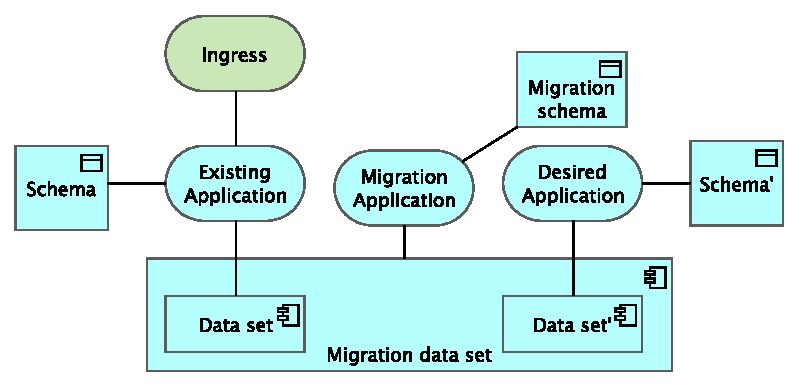
\includegraphics[scale=.8]{figures/migration system deployed.pdf}
   \end{center}
\caption{Migration phase}
\label{fig:migration phase}
\end{figure}
   To automate the migration as much as possible and to achieve zero downtime,
   we must deploy a third system: the migration system.
   This system has its own schema.
   It comprises the schemas of both the existing system and the desired system,
   so the migration system can copy the data from the existing to the desired system.
   It uses transactions to copy the data and to resolve some forms of data pollution.
   Not all migration work, however, can be automated.
   Data pollution, new business rules, or known issues in the existing system
   may occasionally require tailoring the migration script to specific needs
   that require action of users in production.
   For that purpose, the migration engineer specifies business constraints in the migration system.
   In Ampersand, a developer can use business constraints to implement such needs.

   Before a migration starts we assume that the existing system is up and running and all of its invariants are satisfied.
   The ingress is directing traffic to the existing system.
   The data migration has three distinct steps:
\begin{description}
\item[Pre-deploy]
      The migration engineer deploys both the migration system and the desired system with their initial data,
      to allow both systems to satisfy their initial invariants before going live.
      The existing data is still in the existing system and the ingress still directs all traffic to the existing system.
      So, users notice no difference yet.
      The migration system starts copying data from the existing system.
\item[moment of transition (MoT)]
      After the migration system is done copying data, the migration engineer switches all traffic to the migration system.
      This is the moment users will notice the difference because the traffic switch also deploys the functionality of the desired system.
      So, in the eyes of an average user, the migration system may look like the desired system.
      However, the migration system relaxes the blocking invariants of the desired system until users resolve their violations.
      Since the existing system receives no more traffic, its activity will come to a halt and its data will become static.
      The migration system stays active until all invariants of the desired system are satisfied and it can take over the work from the migration system.
\item[moment of completion (MoC)]
      Once the invariants of the desired system are satisfied, the migration engineer switches all traffic to the desired system.
      The blocking invariants of the desired system are now in effect, so users cannot violate them anymore.
      After this switch, the migration engineer can safely remove both the migration system and the existing system.
\end{description}

   Transactions in the existing system that happen during the time that the migration system is copying data cause no problem,
   because their changes are copied by the migration system too.
   However, after the MoT there must be no new changes in the existing system
   to avoid violations of new invariants that the migration system has already fixed.

   The following section introduces the definitions required to migrate data from one system to another.

\section{Definitions}
\label{sct:Definitions}
   An \define{information system} is a combination of data set, schema, and functionality.
   For the purpose of this paper, we ignore functionality captured in user interfaces because it does not impact the migration.
   Section~\ref{sct:Data sets} describes how we define data sets.
   Since data sets are sets, we will use set operators $\cup$ (union), $\cap$ (intersect), $-$ (set difference), and an overline $\cmpl{x}$ as complement operator on sets.
   Section~\ref{sct:Constraints} defines constraints and their violations.
   Schemas are treated in section~\ref{sct:Schemas}.
   Then section~\ref{sct:Information Systems} defines information systems.

\subsection{Data sets}
\label{sct:Data sets}
   A data set $\dataset$ describes a set of structured data, which is typically stored persistently in a database of some kind.
   The notation $\dataset_{\infsys}$ refers to the data set of a particular system $\infsys$.
   The purpose of a data set is to describe the data of a system at one point in time. 
   Before defining data sets, let us first define the constituent notions of atom, concept, relation, and triple.
   
   Atoms serve as data elements.
   %Atoms are values without internal structure of interest, meant to represent atomic data elements (e.g. dates, strings, numbers, etc.) in a database.
   %From a business perspective, atoms represent concrete items of the world,
   %such as \atom{Peter}, \atom{1}, or \atom{the king of France}.
   %By convention throughout the remainder of this paper, variables $a$, $b$, and $c$ represent \emph{atoms}.
   All atoms are taken from an infinite set called $\Atoms$.
   %
   Concepts are names that group atoms of the same type.
   All concepts are taken from an infinite set $\Concepts$.
   %$\Concepts$ and $\Atoms$ are disjoint.
   For example, a developer might choose to classify \atom{Peter} and \atom{Melissa} as \concept{Person},
   and \atom{074238991} as a \concept{TelephoneNumber}.
   In this example, \concept{Person} and \concept{TelephoneNumber} are concepts.
   Moreover, \atom{Peter}, \atom{Melissa} and \atom{074238991} are atoms.
   In the sequel, variables $A$, $B$, $C$, $D$ will represent concepts, and variables $a$, $b$, and $c$ represent \emph{atoms}.
   %
   The relation $\instance:\Pair{\Atoms}{\Concepts}$ relates atoms to concepts.
   The term $a\instance C$ means that atom $a$ is an \emph{instance} of concept $C$.
   %This relation is used in the type system, in which $\instance$ assigns one or more concepts to every atom in the data set.
   %Since $\instance$ is a relation and every relation is a set of pairs,
   %set operators $\cup$, $\cap$, and $-$ can be used on $\instance$.

   Relations serve to organize and store data, allowing developers to represent facts.
   In this paper, variables $r$, $s$, and $d$ represent relations\footnote{Some readers might like to read `relation symbol' where we write `relation'.}.
   All relations are taken from an infinite set $\Rels$.
   $\Rels$ is disjoint from $\Concepts$ and $\Atoms$.
   Every relation $r$ has a name, a source concept, and a target concept.
   The notation $r=\declare{n}{A}{B}$ denotes that relation $r$ has name $n$, source concept $A$, and target concept $B$.
   The part $\pair{A}{B}$ is called the \define{signature} of the relation.
   
   Triples serve to represent data.
   A triple %\footnote{Please note that this paper uses the word {\em triple} in a more restricted way than in natural language.}
   is an element of $\Triple{\Atoms}{\Rels}{\Atoms}$.
   For example, $\triple{\text{\atom{Peter}}}{\declare{\id{phone}}{\tt Person}{\tt TelephoneNumber}}{\text{\atom{074238991}}}$ is a triple.
   
   \begin{definition}[Data set]
   A data set $\dataset$ is a tuple $\pair{\triples}{\instance}$ with finite $\triples \subseteq {\Triple{\Atoms}{\Rels}{\Atoms}}$ and $\instance\subseteq\Pair{\Atoms}{\Concepts}$ that satisfies:
\begin{eqnarray}
   \triple{a}{\declare{n}{A}{B}}{b}\in\triples&\Rightarrow&a\instance A\ \wedge\ b\instance B
\label{eqn:wellTypedEdge}
\end{eqnarray}
\end{definition}
   Looking at the example,
   equation~\ref{eqn:wellTypedEdge} says that \atom{Peter} is an instance of {\tt Person} and \atom{074238991} is an instance of {\tt TelephoneNumber}.
   In practice, users can say that the Person Peter has telephone number 074238991.
   So, the ``thing'' that \atom{Peter} refers to (which is Peter) has \atom{074238991} as a telephone number.
   The notations $\triples_{\dataset}$ and $\instance_{\dataset}$ are used to disambiguate $\triples$ and $\instance$ when necessary.
   To save writing in the sequel, the notation $a\ r\ b$ means that $\triple{a}{r}{b}\in\triples$.

   A relation $r$ can serve as a container of pairs,
   as defined by the function $\popF{r}:\Dataset\rightarrow\powerset{\Pair{\Atoms}{\Atoms}}$.
   It defines a set of pairs, also known as the population of $r$:
\begin{equation}
   \pop{r}{\dataset}\ =\ \{ \pair{a}{b}\mid\ \triple{a}{r}{b}\in\triples_{\dataset}\}
\label{eqn:pop-rel}
\end{equation}
   Note that the phrase ``pair $\pair{a}{b}$ is in relation $r$'' means that there is a dataset $\dataset$ in which $\pair{a}{b}\in\pop{r}{\dataset}$,
   so the phrase ``triple $\triple{a}{r}{b}$ is in $\dataset$'' means the same thing.
%   Equation~\ref{eqn:wellTypedEdge} implies that for every data set $\dataset$:
%\[\pair{a}{b}\in\pop{\declare{n}{A}{B}}{\dataset}\ \Rightarrow\ a\instance_{\dataset}A\ \wedge\ b\instance_{\dataset}B\]
%   For a developer, this means that the type of an atom depends only on the relation in which it resides; not on the actual population of the database.
%
   We overload the notation $\popF{}$ so we can use it on concepts $\popF{C}:\Dataset\rightarrow\powerset{\Atoms}$
   and expressions. We also define the difference of populations, in equation~\ref{eqn:pop-expr}, both for relations and concepts:
\begin{align}
   \pop{C}{\dataset}&= \{ x\mid\ x\ \instance_{\dataset}\ C\}
\label{eqn:pop-concept}\\
   \pop{x-y}{\dataset}&= \pop{x}{\dataset} - \pop{y}{\dataset}
\label{eqn:pop-expr}
\end{align}

\subsection{Constraints}
\label{sct:Constraints}
   Every constraint is an element of an infinite set called $\Constraints$.
   In this paper, variables $u$ and $v$ represent all three types of constraints.
   We say that a constraint, $u$, is satisfied when $u$ is true for all triples in the data set.
   For every constraint $u$, function $\violC{u}:\Dataset\rightarrow\powerset{\Pair{\Atoms}{\Atoms}}$ produces the violations of $u$,
   and $\sign{u}:\Pair{\Concepts}{\Concepts}$ yields the signature of $u$.
   The definition of $\violC{u}$ implies the assumption that we represent each violation as a pair.
   Every constraint must satisfy:
\begin{equation}
   \pair{a}{b}\in\viol{u}{\dataset}\ \wedge\ \sign{u}=\pair{A}{B}\ \Rightarrow\ a\instance A\ \wedge\ b\instance B
\label{eqn:wellTypedViolation}
\end{equation}
   Note that $\viol{u}{\dataset}=\emptyset$ means that $\dataset$ satisfies $u$.

   In case $u$ is a transactional invariant,
   the system will keep it satisfied by adding the violations to a specific relation $\declare{n}{A}{B}$.
\begin{equation}
   \begin{array}[t]{l}
      \viol{u}{\pair{\triples\cup\{\triple{a}{\declare{n}{A}{B}}{b}\mid\pair{a}{b}\in\viol{u}{\dataset}\}}{\instance\cup\instance'}}=\emptyset\\
      \text{\bf with}\ \instance'=\{ \pair{a}{A}\mid\pair{a}{b}\in\viol{u}{\dataset}\}\cup\{ \pair{b}{B}\mid\pair{a}{b}\in\viol{u}{\dataset}\}
   \end{array}
\label{eqn:transaction}
\end{equation}
   It is obvious that not every conceivable constraint can satisfy this equation.
   So, we assume that the compiler restricts the set of transactional invariants to those that satisfy equation~\ref{eqn:transaction}.
   As $\declare{n}{A}{B}$ is specific for $u$, we can write $\enfRel{u}$ for it.
   We call this the \define{enforced relation} of transactional invariant $u$:
\begin{equation}
   \enfRel{u}=\declare{n}{A}{B}
\end{equation}
   Let us denote a transactional invariant as $r\mapsfrom\violC{u}$ or equivalently $r \mapsfrom \lambda \dataset.~\viol{u}{\dataset}$,
   in which $r=\enfRel{u}$.
   
   The language Ampersand has more types of transactional invariants than just this one,
   but this is sufficient for this paper.

\subsection{Schemas}
\label{sct:Schemas}
   Schemas serve to capture the semantics of a system~\cite{Spivak2012}.
   They define concepts, relations, and constraints.
   We assume that a software engineer defines a schema on design time, and a compiler checks whether the semantics are consistent.
   Errors the compiler detects are prohibitive for generating code,
   to prevent a substantial class of mistakes to ever reach end users.

   We describe a schema $\schema$ as a tuple $\quintuple{\concepts}{\rels}{\rules}{\transactions}{\busConstraints}$,
   in which $\concepts\subseteq\Concepts$ is a finite set of concepts,
   $\rels\subseteq\Rels$ is a finite set of relations,
   $\rules\subseteq\Constraints$ is a finite set of blocking invariants,
   $\transactions\subseteq\Constraints$ is a finite set of transactional invariants,
   and $\busConstraints\subseteq\Constraints$ is a finite set of business constraints.

   \begin{definition}[Schema]
   A schema is a tuple $\quintuple{\concepts}{\rels}{\rules}{\transactions}{\busConstraints}$ that satisfies:
\begin{align}
   \declare{n}{A}{B}\in\rels&~\Rightarrow~ A\in\concepts\,\wedge\, B\in\concepts
   \label{eqn:relationsIntroduceConcepts}\\
   u\in\rules\cup\transactions\cup\busConstraints\ \wedge\ \sign{u}=\pair{A}{B}&~\Rightarrow~A\in\concepts\,\wedge\, B\in\concepts\label{eqn:invariant-has-type}\\
   (\declare{n}{A}{B}\mapsfrom t)\in\mathcal\transactions&~\Rightarrow~ \declare{n}{A}{B}\in \rels\label{eqn:enforcement-has-type}
\end{align}
   \end{definition}
   Requirements~\ref{eqn:relationsIntroduceConcepts} and~\ref{eqn:invariant-has-type} ensure that concepts mentioned in relations and in the signature of rules are part of the schema.
   Requirement~\ref{eqn:enforcement-has-type} ensures the enforced relation of a transactional invariant is declared in the schema. 
   When clarity is needed, we write $\concepts_{\schema}$, $\rels_{\schema}$, $\rules_{\schema}$, $\transactions_{\schema}$, $\busConstraints_{\schema}$
   for $\concepts$, $\rels$, $\rules$, $\transactions$, $\busConstraints$ corresponding to $\schema = \quintuple{\concepts}{\rels}{\rules}{\transactions}{\busConstraints}$.

\subsection{Information Systems}
\label{sct:Information Systems}
   Let us now define information systems by enumerating the requirements.
\begin{definition}[information system]
\label{def:information system}
\item An information system $\infsys$ is a tuple $\pair{\dataset}{\schema}$, in which
\begin{itemize}
\item $\dataset=\pair{\triples}{\instance}$ is a data set (so it must satisfy equation~\ref{eqn:wellTypedEdge}).
   We write $\triples_\infsys = \triples$ and $\instance_\infsys = \instance$ if needed;
\item $\schema=\quintuple{\concepts}{\rels}{\rules}{\transactions}{\busConstraints}$ is a schema (so it must satisfy equations~\ref{eqn:relationsIntroduceConcepts} thru~\ref{eqn:enforcement-has-type}).
\item Triples in the data set must have their relation mentioned in the schema:
   \begin{eqnarray}
      \triple{a}{\declare{n}{A}{B}}{b}\in\triples&\Rightarrow&\declare{n}{A}{B}\in\rels
   \label{eqn:define R}
   \end{eqnarray}
\item All violations must have a type, which follows from  (\ref{eqn:wellTypedViolation}).
\item Transactional invariants remain satisfied by adding violations to a specific relation (\ref{eqn:transaction}).
\item All invariants must remain satisfied:
   \begin{align}
      \forall u\in\rules\cup\transactions&.~\viol{u}{\dataset}=\emptyset
   \label{eqn:satisfaction}
   \end{align}
\end{itemize}
\end{definition}
   We assume that a deployment will fail if these requirements are not satisfied.
   We will write $\text{isIS}(\infsys)$ to denote that $\infsys$ is an information system.

\section{Generating a Migration Script}
\label{sct:Generating}
   The complexity of migrating data to date yields expensive and error-prone migration projects.
   By generating this code we can eliminate human induced errors.
   
   This section starts with a presentation of the algorithm.

\subsection{Algorithm for generating a migration script}
   In the migration system, we need to refer to the items (concepts, relations, and constraints) of both the existing system and the desired system.
   We have to relabel items with prefixes to avoid name clashes in the migration system.
   We use a left arrow to denote relabeling by prefixing the name of the item with ``old.''.
\begin{equation}
   \begin{array}[m]{rcl}
      \overleftarrow{\pair{\dataset}{\schema}}&=&\pair{\overleftarrow{\dataset}}{\overleftarrow{\schema}}\\
      \overleftarrow{\pair{\triples}{\instance}}&=&\pair{\overleftarrow{\triples}}{\instance}\\
      \overleftarrow{\quintuple{\concepts}{\rels}{\rules}{\transactions}{\busConstraints}}&=&\quintuple{\concepts}{\overleftarrow{\rels}}{\overleftarrow{\rules}}{\overleftarrow{\transactions}}{\overleftarrow{\busConstraints}}\\
      \overleftarrow{\triples}&=&\{\triple{a}{\overleftarrow{r}}{b}\mid\triple{a}{r}{b}\in\triples\}\\
      \overleftarrow{\declare{n}{A}{B}}&=&\declare{old.n}{A}{B}\\
      \overleftarrow{X}&=&\{\overleftarrow{x}\mid x\in X\}\\
      \viol{\overleftarrow{u}}{\overleftarrow{\dataset}}&=&\viol{u}{\dataset}\\
      \sign{\overleftarrow{u}}&=&\sign{u}\\
      \enfRel{\overleftarrow{u}}&=&\overleftarrow{\enfRel{u}}
   \end{array}
\end{equation}
   The notation $\overrightarrow{\infsys}$ is defined similarly, using prefix ``new.'' instead of ``old.''.

   Then we define the migration system $\migrsys$ as follows:
   Let $\pair{\dataset}{\schema}$ be the existing system.
   Let $\pair{\dataset'}{\schema'}$ be the desired system in its initial state.
\begin{enumerate}
\item We take a disjoint union of the data sets by relabeling relation names, so the migration script can refer to relations from both systems:
   \begin{align}
      \dataset_\migrsys={}&\overleftarrow{\dataset}\cup\overrightarrow{\dataset'}
   \end{align}
\item\label{step2} We create transactional invariants to copy the population of relations from $\dataset$ to $\dataset'$:
   For every relation $r$ shared by the existing and desired systems, we generate a helper relation: ${\tt copy}_r$, and two transactional invariants.
   The first transactional invariant populates relation $\overrightarrow{r}$ and the second populates ${\tt copy}_r$.
   The helper relation ${\tt copy}_r$ contains the pairs that have been copied.
   We use the helper relation to keep the transactional invariants from immediately repopulating $\overrightarrow{r}$ when a user deletes triples in $\dataset'$.
% \begin{verbatim}
%    RELATION copy.r[A*B]
%    RELATION new.r[A*B] [UNI]
%    ENFORCE copy.r >: new.r /\ old.r
%    ENFORCE new.r >: old.r - copy.r
% \end{verbatim}
   \begin{align}
      \rels_1={}&\{{\tt copy}_r\mid r \in \rels_{\schema'}\cap\rels_{\schema}\}\label{eqn:copy relations}\\
      \transactions_1={}&\{\overrightarrow{r}\mapsfrom \popF{\overleftarrow{r}-{\tt copy}_r} \mid r \in\rels_1\}\cup\{{\tt copy}_r\mapsfrom \popF{\overrightarrow{r}\cap\overleftarrow{r}} \mid r \in\rels_1\}
   \end{align}
   The copying process terminates when:
   \begin{align}
      \forall r\in\rels_1.~\overleftarrow{r}={\tt copy}_r\label{eqn:copyingTerminates}
   \end{align}

\item\label{step3}
   The new blocking invariants are $\rules_{\schema'}-\rules_{\schema}$.
   For each new blocking invariant $u$, we generate a helper relation: ${\tt fixed}_u$, to register all violations that are fixed,
   and a blocking invariant $v$ in the migration system that blocks fixed violations from recurring:
% \begin{verbatim}
%    RELATION fixed_TOTr[A*A]
%    RULE Block_TOTr : fixed_TOTr |- new.r;new.r~
%    MESSAGE "Relation r[A*B] must remain total."
%    VIOLATION (TXT "Atom ", SRC I, TXT " must remain paired with an atom from B.")
% \end{verbatim}
   \begin{align}
      \rels_2={}&\{{\tt fixed}_u\mid u \in\overrightarrow{\rules_{\schema'}-\rules_{\schema}}\}\\
      \rules_\text{block}={}&\{v\ 
      \begin{array}[t]{l}
         \text{\bf with}\\
         \sign{v}=\sign{u}\\
         \viol{v}{\dataset}=\viol{u}{\dataset}\cap{\tt fixed}_u
      \end{array}\label{eqn:blockRule}\\
      &\mid u\in\overrightarrow{\rules_{\schema'}-\rules_{\schema}}\}\notag
   \end{align}
   % Note that the blocking invariants from $\schema'\cap\schema$ are also used in $\migrsys$ to ensure continuity.
\item\label{step4}
   We use a transactional invariant to produce the population of the helper relation ${\tt fixed}_u$.
% \begin{verbatim}
%    ENFORCE fixed_TOTr >: I /\ new.r;new.r~
% \end{verbatim}
   \begin{equation}
     \transactions_2\ =\ \{{\tt fixed}_u\mapsfrom\lambda\dataset.~\cmpl{\viol{u}{\dataset}}\mid u\in\overrightarrow{\rules_{\schema'}-\rules_{\schema}}\}\label{eqn:enforceForRules}
   \end{equation}
\item\label{step5} To signal users that there are violations that need to be fixed, we generate a business constraint for each new blocking invariant $u$:
% \begin{verbatim}
%    ROLE User MAINTAINS TOTr
%    RULE TOTr : I |- new.r;new.r~
%    MESSAGE "Please, make relation r[A*B] total."
%    VIOLATION (TXT "Fix ", SRC I, TXT " by pairing it with an (any) atom from B.")
% \end{verbatim}
   \begin{align}
      \busConstraints_\text{fix}={}&\{v\ 
      \begin{array}[t]{l}
         \text{\bf with}\label{eqn:Bfix}\\
         \sign{v}=\sign{u}\\
         \viol{v}{\dataset}=\viol{u}{\dataset}-{\tt fixed}_u
      \end{array}\\
      &\mid u\in\overrightarrow{\rules_{\schema'}-\rules_{\schema}}\}\notag
   \end{align}
   In some cases, a migration engineer can invent ways to satisfy these invariants automatically.
   For this purpose, the generator must produce source code (as opposed to compiled code) to allow the migration engineer
   to replace a business constraint with transactional invariants of her own making.
   After all violations are fixed, i.e. when equation~\ref{eqn:readyForMoC} is satisfied,
   the migration engineer can switch the ingress to the desired system.
   This occurs at MoC and
   replaces $\rules_\text{block}$ in the migration system by the blocking invariants of the desired system.
   This moment arrives when:
   \begin{align}
      \forall u\in\rules_{\schema'}-\rules_{\schema}.~\viol{\overrightarrow{u}}{\dataset}\subseteq{\tt fixed}_u
   \label{eqn:readyForMoC}
   \end{align}
   After this, the migration engineer can remove the migration system and the old system.

\item Let us combine the above into a single migration schema:
   \begin{align}
      \schema_\migrsys=\langle{}&\concepts_\dataset\cup\concepts_{\dataset'},\label{eqn:schema migrsys}\\
      &\overleftarrow{\rels_{\schema}}\cup\overrightarrow{\rels_{\schema'}}\cup\rels_1\cup\rels_2,\notag\\
      &\rules_\text{block}\cup\overrightarrow{\rules_{\schema}\cap\rules_{\schema'}},\notag\\
      &\transactions_1\cup\transactions_2\cup\overrightarrow{\transactions_{\schema'}},\notag\\
      &\busConstraints_\text{fix}\cup\overrightarrow{\busConstraints_{\schema'}}\rangle\notag
   \end{align}
   This schema represents the migration system.
   In our reasoning, we have only used information from the schemas of the existing system and the desired system.
   This shows that it can be generated from these schemas without using any knowledge of the data sets.
\end{enumerate}

\section{Proof of Concept}
\label{sct:PoC}
   By way of proof of concept (PoC), we have built a migration system in Ampersand.
   To demonstrate it in the context of this paper, the existing system, $\pair{\dataset}{\schema}$, is rather trivial.
   It has no constraints and just one relation, $\declare{r}{A}{B}$.
   Its population is $A=\{a_1,a_2,a_3\}$, $B=\{b_1\}$, and $\pop{r}{\dataset}=\{\pair{a_1}{b_1}\}$.
   The schema of the migration system, $\schema_\migrsys$, follows from definition~\ref{eqn:schema migrsys}.
   Figure~\ref{fig:PoC} exhibits four successive screenshots,
   featuring $\overleftarrow{r}$ as {\small\verb#old_r#},
   $\overrightarrow{r}$ as {\small\verb#new_r#}.
\begin{figure}[bht]
   \begin{center}
      \makebox[\textwidth][c]{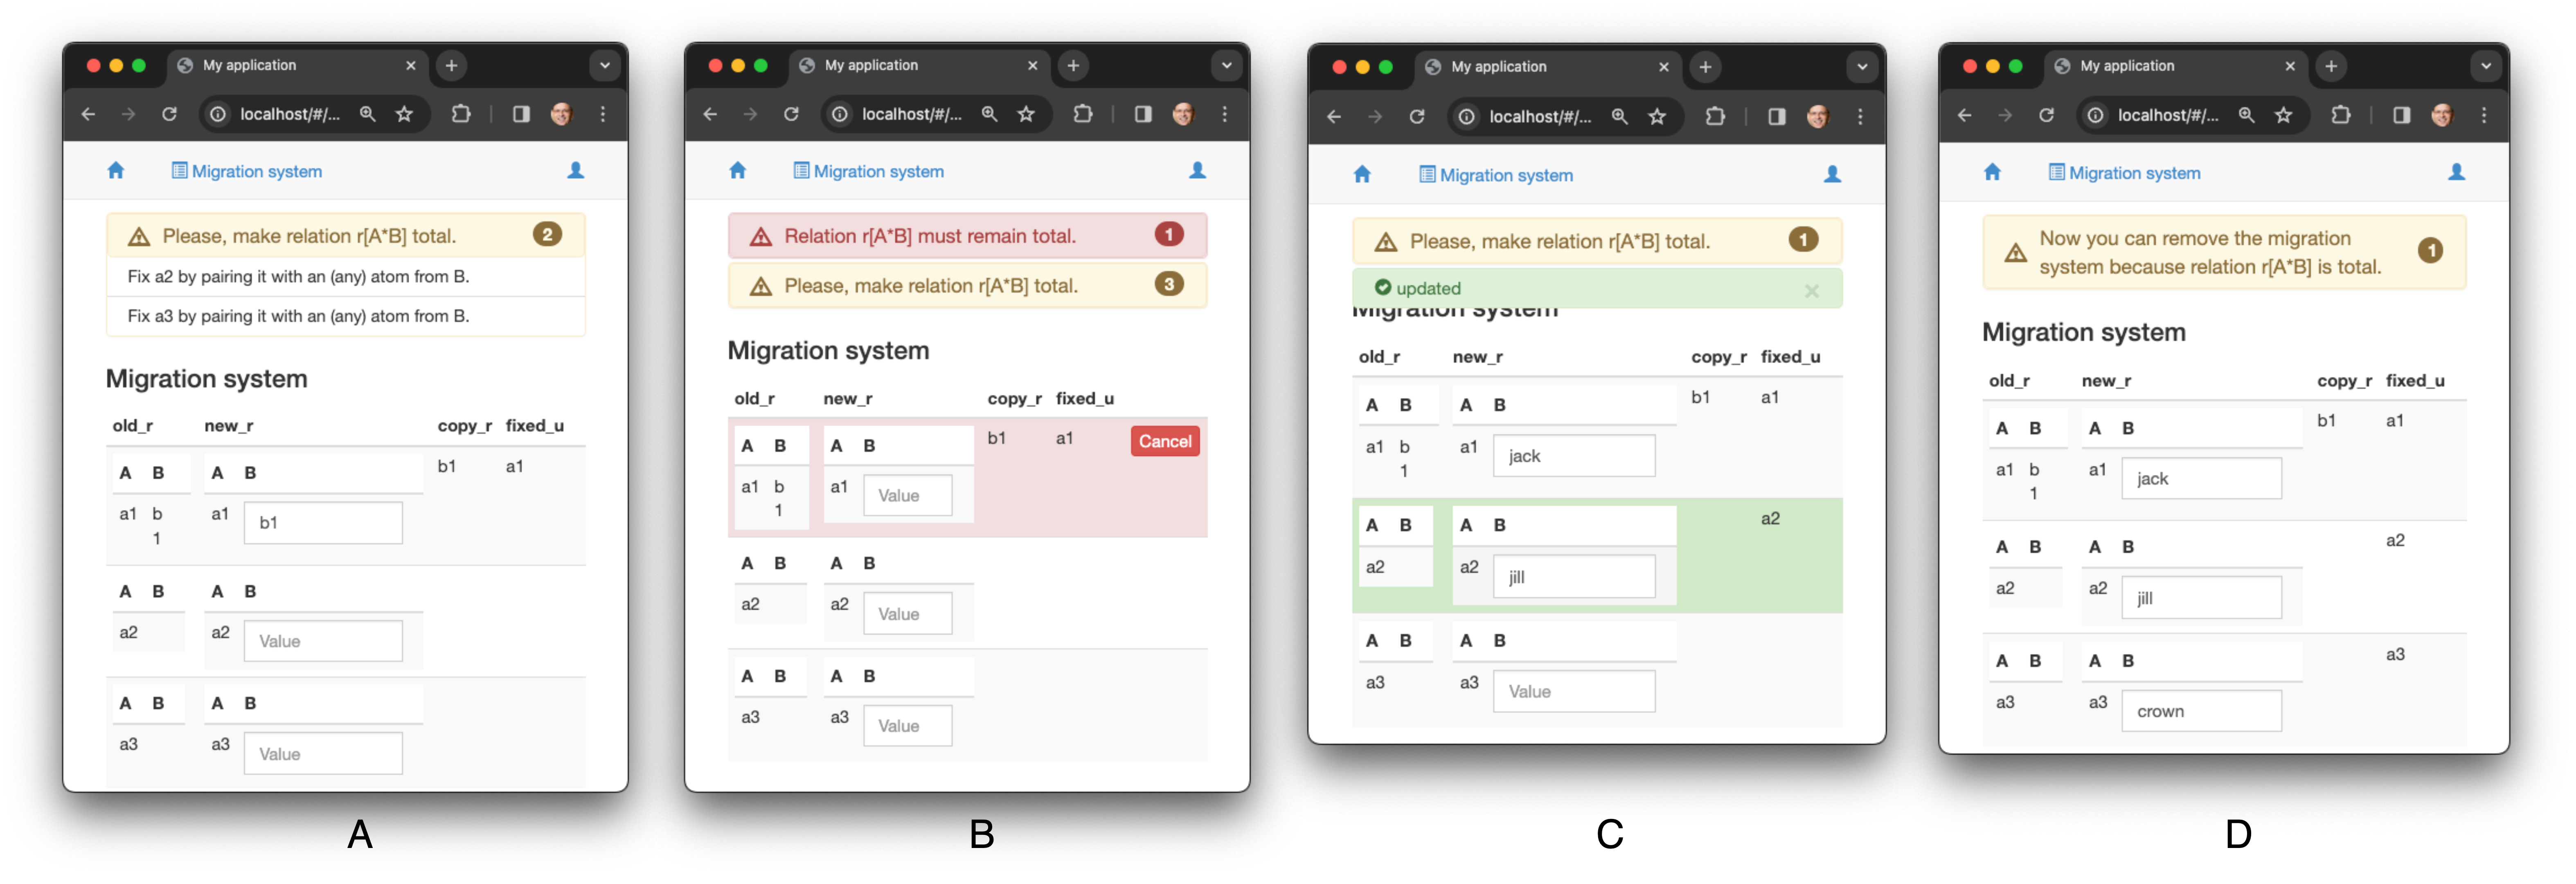
\includegraphics[scale=.07]{figures/screenshots.png}}%
   \end{center}
\caption{Four successive screenshots in the PoC}
\label{fig:PoC}
\end{figure}

   Exhibit A shows the migration system just after deployment, at the MoT.
   It shows that the copying of {\small\verb#old_r#} to {\small\verb#new_r#} has worked.
   The desired system contains one blocking invariant, which is the totality of $\declare{r}{A}{B}$.
   The yellow message in exhibit A indicates that a user needs to fix totality for $a_2$ and $a_3$.
   The column {\small\verb#fixed_u#} contains the elements for which totality is satisfied, so these fields are blocked from becoming empty.

   Exhibit B shows an attempt to remove $\pair{a_1}{b_1}$ from {\small\verb#new_r#}
   The red message blocks this from happening and the user gets a ``Cancel'' button to roll back the action.
   Note that the fields for $a_2$ and $a_3$ are empty, which is fine because they will not be blocked until they are given some value.

   Exhibit C shows that the user fills in ``Jill'', which means that $\pair{a_1}{Jill}$ is added to {\small\verb#new_r#}.
   When the last atom of {tt A} is paired with an atom from {\tt B} (exhibit D), requirement~\ref{eqn:readyForMoC} is satisfied and the prototype informs the user to remove the migration system.

\subsection{Validation}
   The proof of concept gives but one example of something that works.
   To validate that this works in all cases, we must verify that:
\begin{enumerate}
\item The predeployment yields a migration system, $\migrsys$, that copies the designated triples to the desired system in finite time.
\item $\migrsys$ satisfies the definition of information system (\ref{def:information system}) at MoT, especially that it has no violations of blocking invariants (requirement~\ref{eqn:satisfaction}) to ensure a successful deployment.
\item The violations that business actors must fix are finite in number and decrease monotonically, so the business can fulfil the condition for the MoC (requirement~\ref{eqn:readyForMoC}) in finite time.
\item The behavior of $\migrsys$ and the desired system is identical, so moving the ingress from $\migrsys$ to the desired system is not noticable for end-users.
\end{enumerate}
   Let us discuss these points one by one.

   The relations to be copied from the old system are those relations that the desired system retains ($\rels_{\schema'}\cap\rels_{\schema}$).
   For each $r$ to be copied, $\migrsys$ contains a relation ${\tt copy}_r$ in $\rels_1$ (eqn.~\ref{eqn:copy relations}).
   After the MoT, the ingress sends all change events to $\migrsys$, so the existing system can finish the work it is doing for transactional invariants and will not change after that.
   In other words, the population of every relation in $\rels_{\schema}$ becomes stable and so does every ${\tt copy}_r$.
   At that point in time, eqn.~\ref{eqn:copyingTerminates} is true and stays true.
   Effectively, $\transactions_1$ becomes redundant once the copying is done.

   Then, $\migrsys$ contains only blocking invariants that exist in the existing system as well (def.~\ref{dfn:migration system}).
   For this reason, all of these blocking invariants are satisfied on MoT.
   Since $\migrsys$ contains no other blocking invariants, it satisfies requirement~\ref{eqn:satisfaction}.

   Thirdly, the problematic constraints are the blocking invariants of the desired system that were not in the existing system ($\rules_{\schema'}-\rules_{\schema}$ in def.~\ref{eqn:Bfix}).
   The migration engineer might introduce transactional invariants to satisfy these invariants automatically,
   but otherwise, definition~\ref{eqn:Bfix} defines them as business constraints, $\busConstraints_\text{fix}$, to be resolved by the business.
   Each violation in $\busConstraints_\text{fix}$ that a business actor resolves,
   will never reappear because it is registered in ${\tt fixed}_r$ by the transactional invariants of $\transactions_2$ (eqn.~\ref{eqn:enforceForRules}).

   So finally, when all violations are resolved, the constraints in $\busConstraints_\text{fix}$ have effectively become blocking invariants.
   The blocking invariants in the desired system consist of $\rules_{\schema}$ and $\busConstraints_\text{fix}$, which is equivalent to $\rules_{\schema'}$.
   Hence we can replace $\busConstraints_\text{fix}\cup\rules_{\schema}$ with $\rules_{\schema'}$ after condition~\ref{eqn:readyForMoC} is satisfied.

   Now we can assemble the results.
   Every rule in $\rules_\text{block}$ has become blocking, so after the MoC $\rules_\text{block}\cup\overrightarrow{\rules_{\schema}\cap\rules_{\schema'}}=\overrightarrow{\rules_{\schema'}}$ in the migration system, which is $\rules_{\schema'}$ in the desired system.
   Since $\transactions_1$ and $\transactions_2$ are redundant after the MoC,
   we can retain $\overrightarrow{\transactions_{\schema'}}$ in $\migrsys$,
   which is equivalent to $\transactions_{\schema'}$ in the desired system.
   Likewise, $\busConstraints_\text{fix}$ has become redundant, so $\migrsys$ can do with just $\overrightarrow{\busConstraints_{\schema'}}$.
   In the desired system, that is equivalent to $\busConstraints_{\schema'}$.
   So, the constraints in the desired system after the MoC are equivalent to the constraints in the MoC


\section{Conclusions}
\label{sct:Conclusions}
   In this paper, we describe the data migration as going from an existing system to a desired one, where the schema changes.
   As Ampersand generates information systems, creating a new system can be a small task, allowing for incremental deployment of new features.
   We describe the parts of a system that have an effect on data pollution.
   We assume that the existing system does not violate any constraints of its schema, but address other forms of data pollution:
   constraints that are not in the schema but are in the desired schema are initially relaxed such that the business can start using the migration system, after which this form of data pollution needs to be addressed by human intervention.
   We propose a method for doing migration such that only a finite amount of human intervention is needed.
   Our method allows a system similar to the desired system to be used while the intervention takes place.

   Our proposed migration is certainly not the only approach one could think of.
   However, we have not come across other approaches that allow changing the schema in the presence of constraints.
   As such, we cannot compare our approach against other approaches.
   We envision that one day there will be multiple approaches for migration under a changing schema to choose from.
   For now, our next step is to implement the approach shown here into Ampersand.

   This work does not consider what to do about (user) interfaces.
   Instead, it models events by assuming that any change to the data set can be achieved.
   In practice, such changes need to be achieved through interfaces.
   Most Ampersand systems indeed allow the users of the system to edit the data set quite freely through the interfaces.
   However, some interfaces may require certain constraints to be satisfied, which means that interfaces of the desired system might break.
   In the spirit of the approach outlined here, we hope to generate migration interfaces that can replace any broken interfaces until the Moment of Transition.
   How to do this is future work.

%\section{Bibliography}
\bibliographystyle{splncs04}
\bibliography{doc}


\end{document}
